\RequirePackage[T1]{fontenc}  % before the class, so XeTeX never looks for TU/ptm shapes
\documentclass[conference]{IEEEtran}
\usepackage{amsmath,amssymb}
\usepackage{graphicx}
\usepackage{booktabs}
\usepackage{xcolor}
\usepackage{tikz}
\usetikzlibrary{arrows.meta,positioning,fit,calc}
\usepackage{url}
\usepackage[hidelinks]{hyperref}
\newcommand{\TODO}[1]{\textcolor{red}{\textbf{TODO: #1}}}
% generated by figures_scripts/make_values.py; do not edit
\newcommand{\valResClassicalPre}{21.4}
\newcommand{\valResClassicalPost}{21.4}
\newcommand{\valResClassicalCi}{3.9}
\newcommand{\valResClassicalOod}{78.7}
\newcommand{\valResClassicalOodCrash}{34}
\newcommand{\valResLonePre}{15.5}
\newcommand{\valResLonePost}{15.5}
\newcommand{\valResLoneCi}{2.4}
\newcommand{\valResLoneOod}{72.1}
\newcommand{\valResLoneOodCrash}{52}
\newcommand{\valResDrPre}{7.3}
\newcommand{\valResDrPost}{7.3}
\newcommand{\valResDrCi}{1.0}
\newcommand{\valResDrOod}{63.1}
\newcommand{\valResDrOodCrash}{44}
\newcommand{\valResDrftPre}{7.3}
\newcommand{\valResDrftPost}{8.0}
\newcommand{\valResDrftCi}{1.0}
\newcommand{\valResDrftOod}{63.6}
\newcommand{\valResDrftOodCrash}{43}
\newcommand{\valResMamlPre}{8.7}
\newcommand{\valResMamlPost}{7.8}
\newcommand{\valResMamlCi}{1.1}
\newcommand{\valResMamlOod}{70.8}
\newcommand{\valResMamlOodCrash}{49}
\newcommand{\valResFomamlPre}{8.5}
\newcommand{\valResFomamlPost}{7.8}
\newcommand{\valResFomamlCi}{1.0}
\newcommand{\valResFomamlOod}{66.9}
\newcommand{\valResFomamlOodCrash}{46}
\newcommand{\valResAnilPre}{8.6}
\newcommand{\valResAnilPost}{7.7}
\newcommand{\valResAnilCi}{1.1}
\newcommand{\valResAnilOod}{70.4}
\newcommand{\valResAnilOodCrash}{49}
\newcommand{\valResMetasgdPre}{8.7}
\newcommand{\valResMetasgdPost}{7.8}
\newcommand{\valResMetasgdCi}{1.1}
\newcommand{\valResMetasgdOod}{69.3}
\newcommand{\valResMetasgdOodCrash}{48}
\newcommand{\valResReptilePre}{15.2}
\newcommand{\valResReptilePost}{14.8}
\newcommand{\valResReptileCi}{2.0}
\newcommand{\valResReptileOod}{68.6}
\newcommand{\valResReptileOodCrash}{36}
\newcommand{\valResPearlPre}{10.5}
\newcommand{\valResPearlPost}{9.0}
\newcommand{\valResPearlCi}{1.1}
\newcommand{\valResPearlOod}{69.2}
\newcommand{\valResPearlOodCrash}{49}
\newcommand{\valResRltwoPre}{18.4}
\newcommand{\valResRltwoPost}{17.4}
\newcommand{\valResRltwoCi}{1.5}
\newcommand{\valResRltwoOod}{64.6}
\newcommand{\valResRltwoOodCrash}{36}
\newcommand{\valGainClassicalPre}{21.4}
\newcommand{\valGainClassicalPost}{21.4}
\newcommand{\valGainClassicalCi}{3.9}
\newcommand{\valGainClassicalOod}{78.7}
\newcommand{\valGainClassicalOodCrash}{34}
\newcommand{\valGainDrPre}{14.4}
\newcommand{\valGainDrPost}{14.4}
\newcommand{\valGainDrCi}{1.9}
\newcommand{\valGainDrOod}{76.9}
\newcommand{\valGainDrOodCrash}{52}
\newcommand{\valGainDrftPre}{14.4}
\newcommand{\valGainDrftPost}{14.2}
\newcommand{\valGainDrftCi}{1.9}
\newcommand{\valGainDrftOod}{75.5}
\newcommand{\valGainDrftOodCrash}{50}
\newcommand{\valGainMamlPre}{15.6}
\newcommand{\valGainMamlPost}{13.7}
\newcommand{\valGainMamlCi}{2.7}
\newcommand{\valGainMamlOod}{69.8}
\newcommand{\valGainMamlOodCrash}{42}
\newcommand{\valGainFomamlPre}{15.7}
\newcommand{\valGainFomamlPost}{13.9}
\newcommand{\valGainFomamlCi}{2.8}
\newcommand{\valGainFomamlOod}{72.6}
\newcommand{\valGainFomamlOodCrash}{46}
\newcommand{\valGainMetasgdPre}{15.6}
\newcommand{\valGainMetasgdPost}{11.3}
\newcommand{\valGainMetasgdCi}{2.0}
\newcommand{\valGainMetasgdOod}{69.9}
\newcommand{\valGainMetasgdOodCrash}{45}
\newcommand{\valGainReptilePre}{13.5}
\newcommand{\valGainReptilePost}{13.4}
\newcommand{\valGainReptileCi}{1.7}
\newcommand{\valGainReptileOod}{75.4}
\newcommand{\valGainReptileOodCrash}{52}
\newcommand{\valNavClassicalPre}{86}
\newcommand{\valNavClassicalPost}{86}
\newcommand{\valNavClassicalColl}{12}
\newcommand{\valNavClassicalOod}{14}
\newcommand{\valNavClassicalFullPre}{83}
\newcommand{\valNavClassicalFullPost}{83}
\newcommand{\valNavClassicalFullColl}{0}
\newcommand{\valNavClassicallonePre}{81}
\newcommand{\valNavClassicallonePost}{81}
\newcommand{\valNavClassicalloneColl}{18}
\newcommand{\valNavClassicalloneOod}{11}
\newcommand{\valNavClassicalloneFullPre}{75}
\newcommand{\valNavClassicalloneFullPost}{75}
\newcommand{\valNavClassicalloneFullColl}{0}
\newcommand{\valNavDrPre}{82}
\newcommand{\valNavDrPost}{82}
\newcommand{\valNavDrColl}{18}
\newcommand{\valNavDrOod}{15}
\newcommand{\valNavDrFullPre}{67}
\newcommand{\valNavDrFullPost}{67}
\newcommand{\valNavDrFullColl}{33}
\newcommand{\valNavDrftPre}{82}
\newcommand{\valNavDrftPost}{72}
\newcommand{\valNavDrftColl}{28}
\newcommand{\valNavDrftOod}{21}
\newcommand{\valNavDrftFullPre}{67}
\newcommand{\valNavDrftFullPost}{67}
\newcommand{\valNavDrftFullColl}{33}
\newcommand{\valNavEtoePre}{50}
\newcommand{\valNavEtoePost}{50}
\newcommand{\valNavEtoeColl}{50}
\newcommand{\valNavEtoeOod}{7}
\newcommand{\valNavEtoeFullPre}{42}
\newcommand{\valNavEtoeFullPost}{42}
\newcommand{\valNavEtoeFullColl}{58}
\newcommand{\valNavEtoeftPre}{50}
\newcommand{\valNavEtoeftPost}{45}
\newcommand{\valNavEtoeftColl}{55}
\newcommand{\valNavEtoeftOod}{9}
\newcommand{\valNavEtoeftFullPre}{42}
\newcommand{\valNavEtoeftFullPost}{42}
\newcommand{\valNavEtoeftFullColl}{58}
\newcommand{\valNavMamlPre}{79}
\newcommand{\valNavMamlPost}{45}
\newcommand{\valNavMamlColl}{52}
\newcommand{\valNavMamlOod}{7}
\newcommand{\valNavMamlFullPre}{58}
\newcommand{\valNavMamlFullPost}{58}
\newcommand{\valNavMamlFullColl}{42}
\newcommand{\valNavFomamlPre}{80}
\newcommand{\valNavFomamlPost}{36}
\newcommand{\valNavFomamlColl}{61}
\newcommand{\valNavFomamlOod}{8}
\newcommand{\valNavFomamlFullPre}{58}
\newcommand{\valNavFomamlFullPost}{75}
\newcommand{\valNavFomamlFullColl}{25}
\newcommand{\valNavAnilPre}{83}
\newcommand{\valNavAnilPost}{47}
\newcommand{\valNavAnilColl}{50}
\newcommand{\valNavAnilOod}{8}
\newcommand{\valNavAnilFullPre}{67}
\newcommand{\valNavAnilFullPost}{50}
\newcommand{\valNavAnilFullColl}{50}
\newcommand{\valNavMetasgdPre}{76}
\newcommand{\valNavMetasgdPost}{42}
\newcommand{\valNavMetasgdColl}{52}
\newcommand{\valNavMetasgdOod}{6}
\newcommand{\valNavMetasgdFullPre}{75}
\newcommand{\valNavMetasgdFullPost}{33}
\newcommand{\valNavMetasgdFullColl}{58}
\newcommand{\valNavReptilePre}{80}
\newcommand{\valNavReptilePost}{62}
\newcommand{\valNavReptileColl}{38}
\newcommand{\valNavReptileOod}{17}
\newcommand{\valNavReptileFullPre}{58}
\newcommand{\valNavReptileFullPost}{50}
\newcommand{\valNavReptileFullColl}{50}
\newcommand{\valNavPearlPre}{65}
\newcommand{\valNavPearlPost}{66}
\newcommand{\valNavPearlColl}{33}
\newcommand{\valNavPearlOod}{7}
\newcommand{\valNavPearlFullPre}{67}
\newcommand{\valNavPearlFullPost}{17}
\newcommand{\valNavPearlFullColl}{83}
\newcommand{\valNavRltwoPre}{55}
\newcommand{\valNavRltwoPost}{71}
\newcommand{\valNavRltwoColl}{28}
\newcommand{\valNavRltwoOod}{12}
\newcommand{\valNavRltwoFullPre}{33}
\newcommand{\valNavRltwoFullPost}{50}
\newcommand{\valNavRltwoFullColl}{50}
\newcommand{\valTaskMassTrainLo}{0.85}
\newcommand{\valTaskMassTrainHi}{1.30}
\newcommand{\valTaskMassOodLo}{1.30}
\newcommand{\valTaskMassOodHi}{1.40}
\newcommand{\valTaskMotorTrainLo}{75}
\newcommand{\valTaskMotorTrainHi}{100}
\newcommand{\valTaskMotorOodLo}{65}
\newcommand{\valTaskMotorOodHi}{75}
\newcommand{\valTaskDragTrainLo}{0.5}
\newcommand{\valTaskDragTrainHi}{2.0}
\newcommand{\valTaskDragOodLo}{2.0}
\newcommand{\valTaskDragOodHi}{3.0}
\newcommand{\valTaskWindTrainLo}{0.0}
\newcommand{\valTaskWindTrainHi}{2.5}
\newcommand{\valTaskWindOodLo}{2.5}
\newcommand{\valTaskWindOodHi}{4.0}
\newcommand{\valTaskGustTrainLo}{0.0}
\newcommand{\valTaskGustTrainHi}{0.8}
\newcommand{\valTaskGustOodLo}{0.8}
\newcommand{\valTaskGustOodHi}{1.5}
\newcommand{\valTaskLatTrainLo}{0}
\newcommand{\valTaskLatTrainHi}{30}
\newcommand{\valTaskLatOodLo}{30}
\newcommand{\valTaskLatOodHi}{50}
\newcommand{\valResRatioClassical}{2.9}
\newcommand{\valResRatioLone}{2.1}
\newcommand{\valResOodCrashLearnedLo}{43}
\newcommand{\valResOodCrashLearnedHi}{49}
\newcommand{\valOodRmseMin}{63.1}
\newcommand{\valOodAdaptMaxDelta}{6}
\newcommand{\valNavOodMax}{21}
\newcommand{\valNavFullLearnedLo}{17}
\newcommand{\valNavFullLearnedHi}{75}
\newcommand{\valNavFullCollLo}{25}
\newcommand{\valNavFullCollHi}{83}


\begin{document}

\title{Where Does Meta-Learning Help a Quadrotor?\\A Simulation Study of Seven Algorithms\\with Classical Control and Planning}

\author{\IEEEauthorblockN{Amal Mehta}
\IEEEauthorblockA{\TODO{affiliation}\\amal.mehta@gmail.com}}

\maketitle

\begin{abstract}
A quadrotor deployed outside the lab meets conditions it was not tuned for: extra payload, a worn motor, wind and command latency. Meta-reinforcement learning promises adaptation from a few flights, while classical stacks built on geometric control, adaptive control, occupancy mapping and A* planning are dependable but fixed. We ask where meta-learning actually helps when it is combined with such a stack. In one simulator parameterised after a Holybro X500 V2, we insert learning at three points: a residual on the geometric controller, the controller's gains, and the local planner of a depth-camera, mapping and A* navigation stack. We compare seven algorithms (MAML, FOMAML, ANIL, Meta-SGD, Reptile, PEARL and RL$^2$) with nominal, L1-adaptive, domain-randomised and fine-tuning baselines on held-out and out-of-distribution dynamics. A learned residual cuts held-out tracking error from \valResLonePost\,cm with L1 adaptation to \valResDrPost\,cm, but gradient-based adaptation adds little beyond domain randomisation. Meta-learning helps most when it tunes classical gains (Meta-SGD: \valGainMetasgdPre\ to \valGainMetasgdPost\,cm). In navigation, gradient-based adaptation degrades learned planners while RL$^2$ improves with experience, and the classical planner remains the most reliable on the full stack in unseen rooms. Outside the training distribution every method fails, and learned residuals crash more often than the plain controller. We release the suite and recommend a hardware platform and staged plan for real-world tests.
\end{abstract}

\section{Introduction}

Small aerial robots rarely fly the vehicle they were tuned on. A delivery adds payload, a propeller chips, the wind picks up and the companion computer adds latency. Classical control handles part of this: a geometric tracking controller~\cite{lee2010geometric} with integral action rejects slow disturbances, and L1 adaptive augmentation estimates and cancels a lumped disturbance online~\cite{wu2022l1quad}. Learning-based adaptation promises more: meta-learning trains a model that adapts from a few samples of a new task~\cite{finn2017maml}, and learned adaptation has produced agile flight in strong winds~\cite{oconnell2022neuralfly} and single controllers for very different quadrotors~\cite{zhang2022nearhover,eschmann2025raptor}.

Two questions remain open. First, meta-reinforcement-learning algorithms are typically evaluated against each other on simulated robot benchmarks such as locomotion and manipulation suites~\cite{yu2019metaworld,beck2025tutorial}, rather than against the classical controllers and planners that would run in the same loop. Second, a deployed autonomy stack has several places where learning could enter (the low-level controller, its gains, the local planner), and it is not clear which of them benefits from meta-learning.

We study both questions in one simulation suite. A batched quadrotor model parameterised after a Holybro X500 V2 runs a classical stack: a geometric controller with collective-thrust and body-rate (CTBR) output, a simulated RealSense D435i depth camera, a log-odds occupancy map and an A* planner (Fig.~\ref{fig:pipeline}). Meta-learning plugs into three places: a residual on the controller, the controller's gains, and the local planner. Each must adapt to a new task drawn from payload, motor wear, drag, wind, gusts and latency.

Our contributions are:
\begin{itemize}
\item an open simulation suite with three classical+meta combinations and a reproducible benchmark protocol (Secs.~\ref{sec:problem}--\ref{sec:protocol});
\item a comparison of seven meta-learning algorithms with nominal, L1-adaptive, domain-randomised (DR) and fine-tuning baselines on held-out and out-of-distribution (OOD) tasks (Sec.~\ref{sec:results});
\item four findings: a learned residual beats tuned classical adaptation; meta-learning helps most when it adapts classical gains; gradient-based adaptation at the meta-trained step size degrades learned navigation planners, and the classical planner stays the most reliable on the full stack; and no method survives the OOD tasks;
\item a hardware recommendation and staged sim-to-real plan for testing the stack (Sec.~\ref{sec:platform}).
\end{itemize}
Code, results and a replay of recorded flights are available at \url{https://github.com/amalmehta/DroneAutonomy}.

\begin{figure*}[t]
\centering
% Fig. 1: the stack and the three places meta-learning plugs in (hand-drawn TikZ, no data)
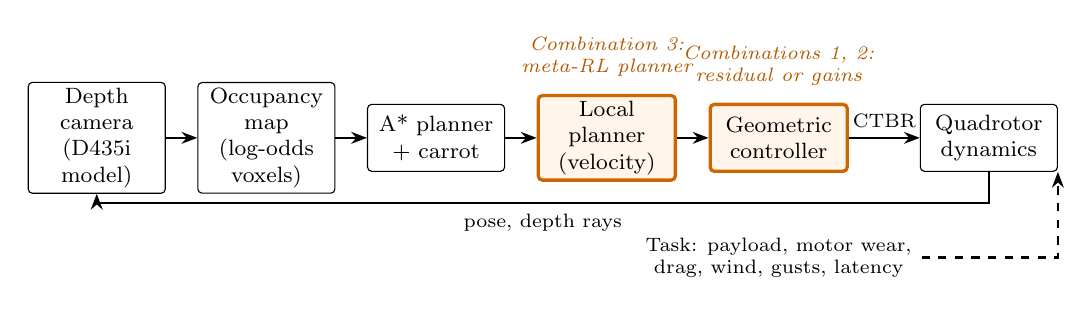
\begin{tikzpicture}[
  box/.style={draw, rounded corners=1.5pt, align=center, font=\footnotesize, minimum height=8.5mm, inner sep=2pt, text width=16mm},
  learn/.style={box, draw=orange!80!black, very thick, fill=orange!8},
  arr/.style={-{Stealth[length=2mm]}, thick},
  tag/.style={font=\scriptsize\itshape, text=orange!70!black, align=center}]
  \node[box] (cam) {Depth camera\\(D435i model)};
  \node[box, right=4mm of cam] (map) {Occupancy map\\(log-odds voxels)};
  \node[box, right=4mm of map] (astar) {A* planner\\+ carrot};
  \node[learn, right=4mm of astar] (local) {Local planner\\(velocity)};
  \node[learn, right=4mm of local] (ctrl) {Geometric\\controller};
  \node[box, right=9mm of ctrl] (dyn) {Quadrotor\\dynamics};
  \draw[arr] (cam) -- (map); \draw[arr] (map) -- (astar); \draw[arr] (astar) -- (local);
  \draw[arr] (local) -- (ctrl);
  \draw[arr] (ctrl) -- node[above, font=\scriptsize] {CTBR} (dyn);
  \draw[arr] (dyn.south) -- ++(0,-4mm) -| node[pos=0.25, below, font=\scriptsize] {pose, depth rays} (cam.south);
  \node[tag, above=1mm of local] {Combination 3:\\meta-RL planner};
  \node[tag, above=1mm of ctrl] {Combinations 1, 2:\\residual or gains};
  \node[font=\scriptsize, align=center, below=7mm of ctrl] (task) {Task: payload, motor wear,\\drag, wind, gusts, latency};
  \draw[arr, dashed] (task.east) -| (dyn.south east);
\end{tikzpicture}

\caption{Meta-learning plugs into three places of one classical stack. The local planner (Combination 3) turns depth and a carrot point on the A* path into a velocity command. The geometric controller turns that into collective thrust and body rates, with a learned residual (Combination 1) or meta-learned gains (Combination 2). The task perturbs the dynamics.}
\label{fig:pipeline}
\end{figure*}

\section{Related Work}

\textbf{Meta-reinforcement learning.} Gradient-based methods learn an initialisation from which a few policy-gradient steps adapt to a new task: MAML~\cite{finn2017maml}, its first-order approximation FOMAML, Reptile~\cite{nichol2018reptile}, ANIL, which adapts only the output layer~\cite{raghu2020anil}, and Meta-SGD, which also learns per-parameter step sizes~\cite{li2017metasgd}. Context-based methods instead infer the task from experience: PEARL encodes recent transitions into a latent variable for an off-policy actor-critic~\cite{rakelly2019pearl}, and RL$^2$ uses a recurrent policy whose state carries what it has learned across episodes~\cite{duan2016rl2,wang2016learning}. These are usually compared with each other on simulated locomotion; we compare them inside a classical flight stack and against classical adaptive control.

\textbf{Learned adaptation for flight.} Neural-Fly learns wind-invariant features offline and adapts a linear layer online~\cite{oconnell2022neuralfly}; adaptive-control-oriented meta-learning trains features for an adaptive law~\cite{richards2021acml}; rapid motor adaptation infers latent dynamics from history~\cite{kumar2021rma}, an idea carried to quadrotors of very different sizes~\cite{zhang2022nearhover}. Domain randomisation trains a single robust policy instead~\cite{tobin2017domain,peng2018dynamics,molchanov2019sim2multireal}. L1 adaptive augmentation of a geometric controller is a strong classical alternative~\cite{wu2022l1quad}. We include domain-randomised and L1 baselines next to the meta-learners.

\textbf{Residual and hybrid control.} Residual RL learns a correction on top of a fixed controller~\cite{johannink2019residual,silver2018residual}. Our Combinations 1 and 2 are residual and gain-tuning variants of this idea, trained with meta-learning.

\textbf{Learned versus classical navigation.} Classical stacks build a map, for example an OctoMap~\cite{hornung2013octomap}, and plan on it with search such as A*~\cite{hart1968astar}. Learned policies can fly fast through clutter from depth alone~\cite{loquercio2021wild}, and RL can outperform optimal control in racing~\cite{song2023reaching}. We keep the map and planner and ask whether a meta-learned local planner improves on a classical one. Open simulators and platforms for learning-based flight include gym-pybullet-drones~\cite{panerati2021pybullet} and Agilicious~\cite{foehn2022agilicious}.

\section{System}\label{sec:system}

\subsection{Vehicle model}
We simulate many drones at once, each with its own task, in a batched rigid-body model integrated at 500\,Hz. Commands are collective thrust and body rates (CTBR), the setpoint PX4 accepts in offboard mode~\cite{meier2015px4}. Each command passes through a latency buffer, then a PX4-like body-rate PI loop that uses the \emph{nominal} inertia, then an X-configuration mixer that gives up yaw torque first when motors saturate. First-order motors (time constant 40\,ms) are scaled by per-motor efficiencies. Forces include linear drag (0.3\,N\,s/m), steady wind and Ornstein--Uhlenbeck gusts. The nominal vehicle approximates a Holybro X500 V2 carrying a Jetson and a D435i: mass 2.0\,kg, arm 0.25\,m and inertia 0.0217/0.0217/0.040\,kg\,m$^2$ from PX4's x500 simulation model; the thrust-to-weight ratio of 2.1, motor lag and drag are our estimates (Sec.~\ref{sec:platform}).

\subsection{Tasks}
A task fixes payload (mass scale; inertia grows by half the relative mass increase, as for a payload near the centre), the efficiency of one randomly chosen motor, drag, steady wind, gust intensity and command latency (Table~\ref{tab:tasks}). Training and held-out tasks share ranges but use disjoint random seeds. OOD tasks lie beyond every range at once.

\begin{table}[t]
\centering
\caption{Task distribution. Each task draws every parameter from the given range.}
\label{tab:tasks}
\footnotesize
% generated by figures_scripts/task_table.py; do not edit
\begin{tabular}{@{}llll@{}}
\toprule
Parameter & Unit & Train / held-out & OOD \\
\midrule
Payload (mass scale) & $\times$ & 0.85--1.30 & 1.30--1.40 \\
Weakest motor efficiency & \% & 75--100 & 65--75 \\
Drag scale & $\times$ & 0.5--2.0 & 2.0--3.0 \\
Steady wind & m/s & 0.0--2.5 & 2.5--4.0 \\
Gust std.\ (OU, 0.5 s) & m/s & 0.0--0.8 & 0.8--1.5 \\
Command latency & ms & 0--30 & 30--50 \\
\bottomrule
\end{tabular}

\end{table}

\subsection{Classical control}
A geometric controller~\cite{lee2010geometric} runs at 100\,Hz: a PID position loop produces a desired acceleration, limited to 35$^\circ$ tilt, which sets collective thrust and an attitude whose error gives body-rate commands. It has seven gains: proportional, derivative and integral gains for the horizontal and vertical axes, and an attitude gain. The adaptive baseline adds piecewise-constant L1 augmentation~\cite{wu2022l1quad}: a velocity predictor estimates a lumped acceleration disturbance, whose low-pass-filtered value is subtracted from the desired acceleration.

\textbf{Tracking.} Combinations 1 and 2 are scored on trajectory tracking: each episode follows a smooth random reference (a sum of two cosines per axis, at most 2\,m/s horizontally; 15\% of episodes are pure hover) for 4\,s. The reward is $\exp(-\|e\|/0.25)$ for position error $e$ in metres, minus a small action penalty. An episode ends early if the error exceeds 1.5\,m or the tilt exceeds 70$^\circ$.

\textbf{Combination 1: residual on the controller.} At 50\,Hz a policy adds a bounded correction to the controller's output: up to 25\% of hover thrust, and up to 1\,rad/s in roll and pitch rate (0.5\,rad/s in yaw). It observes tracking errors, velocity, attitude, body rates, the reference acceleration, its previous action and the controller's own command.

\textbf{Combination 2: controller gains.} The policy is a Gaussian over the logarithm of the seven gain scales relative to nominal. One gain vector is drawn per episode and the controller flies the whole episode with it.

\subsection{Navigation stack (Combination 3)}
Rooms measure 14$\times$8$\times$3\,m and contain randomly placed pillars and boxes; a quarter of the boxes hang from the ceiling with their lowest edge at 1.9\,m or higher, so the map and planner work in three dimensions. Start and goal sit at opposite ends. The drone is a 0.35\,m sphere for collision checks.

\textbf{Perception and mapping.} A depth camera modelled on the D435i casts rays over an 87$^\circ\times$58$^\circ$ field of view up to 5\,m, adds noise with standard deviation $0.008\,d^2$ and drops 2\% of pixels. The policy sees a 16$\times$8 image; the mapper uses 48$\times$24. A log-odds voxel map with 0.2\,m voxels carves free space along each ray, stopping one voxel short of a hit so that grazing rays don't erase surfaces.

\textbf{Planning.} A* searches the 26-connected voxel grid inflated by the drone radius plus a 0.15\,m margin, replanned at 2\,Hz. The carrot is the furthest point up to 1.5\,m along the path that is still in straight-line sight.

\textbf{Local planner.} At 10\,Hz the local planner outputs a velocity command in the heading frame. The classical controller tracks it through a leashed position setpoint while yaw turns toward the carrot. The learned planner observes the depth image, the carrot and goal in the heading frame, velocity, attitude, altitude and its previous action. It is rewarded for progress along the true shortest path, with penalties for time, proximity, jerky commands and collisions, and a bonus at the goal. The classical local planner pursues the carrot, slows down near depth returns and adds a repulsive term from close returns. For speed, learned planners are trained with a privileged planner: a distance field computed on the true map, equivalent to A* on a perfect map. Evaluation also runs the full online stack.

\section{Learners and Baselines}\label{sec:learners}

All step policies are Gaussian MLPs (64--64 units for tracking, 128--64 for navigation) with a state-independent standard deviation. To keep differences down to the meta-learning rule, the gradient-based methods share one estimator: per-task linear feature baselines with generalised advantage estimation~\cite{schulman2015gae} and PPO-clipped updates~\cite{schulman2017ppo}.

\textbf{MAML family.} Each iteration samples 16 tasks and flies 10 episodes per task. One vanilla policy-gradient step with step size 0.1 adapts the policy to each task; all tasks adapt in one batched backward pass. The adapted policies fly 10 new episodes, and a PPO-clipped outer loss on those episodes is backpropagated through the adaptation step. MAML~\cite{finn2017maml} differentiates through the inner gradient (second order); FOMAML drops that term; ANIL adapts only the output layer and the standard deviation~\cite{raghu2020anil}; Meta-SGD also learns a step size for every parameter~\cite{li2017metasgd}. Like the original MAML for RL, we ignore how the pre-adaptation sampling distribution depends on the parameters~\cite{rothfuss2018promp}.

\textbf{Reptile}~\cite{nichol2018reptile} runs three rounds of per-task PPO (Adam, four epochs per round), each on fresh episodes, then moves the shared parameters toward the mean adapted parameters with a step that anneals from 0.5 to 0.1.

\textbf{PEARL}~\cite{rakelly2019pearl} trains a soft actor-critic~\cite{haarnoja2018sac} conditioned on a five-dimensional latent task variable. A permutation-invariant encoder maps transitions from 32 training tasks to a product-of-Gaussians posterior, trained through the critic loss plus a KL penalty to the prior.

\textbf{RL$^2$}~\cite{duan2016rl2,wang2016learning} uses a GRU policy with 128 units that sees the previous action, reward and an episode-start flag, and keeps its hidden state over a trial of three episodes on the same task. It is trained with recurrent PPO over whole trials.

\textbf{Baselines.} \emph{Classical} uses nominal gains and no learning; \emph{Classical + L1} adds L1 augmentation. \emph{DR} trains one policy with PPO over the whole task distribution (domain randomisation) and never adapts; \emph{DR + fine-tune} adapts it at test time with the same per-task PPO rounds as Reptile. For Combination 2 the DR baseline is the same Gaussian over gains, trained over all tasks without a meta objective. For navigation we add \emph{end-to-end DR}, a DR planner that sees the goal direction instead of the carrot, with no map or planner.

\textbf{Training budgets.} Table~\ref{tab:budget} lists the training budget of each learner. DR and the MAML family saw the same data on tracking, while PEARL and RL$^2$ saw less.

\begin{table}[t]
\centering
\caption{Training budget in millions of environment steps.}
\label{tab:budget}
\footnotesize
% generated by figures_scripts/budget_table.py; do not edit
\begin{tabular}{@{}lrrrrr@{}}
\toprule
Combination & DR & MAML fam. & Reptile & PEARL & RL$^2$ \\
\midrule
C1 residual & 9.6 & 9.6 & 11.5 & 1.0 & 4.3 \\
C2 gains & 4.8 & 6.4 & 7.7 & -- & -- \\
C3 planner$^*$ & 12.0 & 5.8 & 7.2 & 1.0 & 5.2 \\
\bottomrule
\multicolumn{6}{@{}l}{$^*$MAML family and Reptile: additional steps after starting from DR.}
\end{tabular}

\end{table}

\textbf{Navigation specifics.} Training navigation planners from scratch is the most expensive part of the study, so to fit our CPU budget the gradient-based meta-learners start from the trained DR planner and meta-train from there. PEARL and RL$^2$ use different networks and train from scratch, so their comparison with the others is confounded by starting point. With the tracking step size (Adam, 3e-3), per-task PPO adaptation wrecked the warm-started navigation planner (Reptile reached 0\% success), so navigation uses 3e-4 for both Reptile and DR + fine-tune; the diverged run is kept in the released results.

\section{Experimental Protocol}\label{sec:protocol}

\textbf{Tasks and rooms.} Every method is scored on fixed task sets: 32 held-out and 32 OOD tasks for tracking, and 24 of each for navigation. Navigation episodes are flown in rooms from a test pool of 128 that is never used in training, each episode in its own room (\valNavPrivRooms\ rooms per seed).

\textbf{Adaptation.} Before adapting and after each of three adaptation stages, we fly four deterministic evaluation episodes (the policy mean) per task. A stage of gradient-based adaptation uses 10 exploratory episodes and one update, so three stages use 30 episodes. The MAML family is meta-trained for a single update, so stages 2 and 3 extrapolate beyond the trained procedure; where it matters we also report the one-update result. A PEARL stage adds one episode of context, and an RL$^2$ stage is one more episode of the trial. Non-adapting methods are evaluated once.

\textbf{Full stack.} Navigation is scored twice. Learned planners are first scored with the privileged planner, and every method is then scored on the full online stack (depth camera, map built in flight, A*) in \valNavFullRooms\ unseen rooms per seed, before and after one adaptation stage. The stage's exploration flights use the privileged planner, like a calibration flight in a known room.

\textbf{Metrics and statistics.} We report tracking RMSE in centimetres, with an early termination counting as 1.5\,m error for the rest of the episode, and navigation success: reaching within 0.5\,m of the goal before a collision or a 30\,s time-out. Learned methods are trained with \valSeedsRes\ seeds on the residual problem, \valSeedsGain\ on the gain problem and \valSeedsNav\ on navigation; intervals are 95\% normal intervals over tasks and seeds. Paired comparisons use the same tasks and seeds for both methods, with bootstrap intervals over task--seed pairs. Everything ran on one shared Intel Core i9-9980HK CPU without a GPU.

\section{Results}\label{sec:results}

We organise the results around four questions: does learning beat classical adaptation for tracking (\ref{sec:rq1}), where does meta-learning add to it (\ref{sec:rq2}), what happens when a learned planner adapts inside the navigation stack (\ref{sec:rq3}), and how do methods behave beyond the training distribution (\ref{sec:rq4}).

\begin{table*}[t]
\centering
\caption{Tracking under new dynamics. A learned residual roughly halves the error of classical adaptation, and meta-learning helps most when it tunes the controller's gains. Held-out RMSE before and after adapting (mean, with the 95\% half-interval after adapting), OOD RMSE and OOD crash rate after adapting. Data: adaptation episodes used. Bold: best in column. Residual learners use \valSeedsRes\ training seeds, gain learners \valSeedsGain.}
\label{tab:tracking}
\footnotesize
% generated by figures_scripts/tracking_table.py; do not edit
\begin{tabular}{@{}llrrrrrrr@{}}
\toprule
 & & \multicolumn{4}{c}{Combination 1: residual on controller} & \multicolumn{3}{c}{Combination 2: controller gains} \\
\cmidrule(lr){3-6}\cmidrule(l){7-9}
Method & Data & Before & After & OOD & OOD crash & Before & After & OOD \\
 & (ep.) & (cm) & (cm) & (cm) & (\%) & (cm) & (cm) & (cm) \\
\midrule
\multicolumn{9}{@{}l}{\emph{Classical}} \\
Classical (nominal gains) & 0 & 21.4 & 21.4 & 78.7 & \textbf{34} & 21.4 & 21.4 & 78.7 \\
Classical + L1 & 0 & 15.5 & 15.5 & 72.1 & 52 & -- & -- & -- \\
\multicolumn{9}{@{}l}{\emph{Non-meta learned}} \\
DR (no adapt.) & 0 & \textbf{7.3} & \textbf{7.3} & \textbf{63.1} & 44 & 14.4 & 14.4 & 76.9 \\
DR + fine-tune & 30 & \textbf{7.3} & 8.0{\scriptsize$\pm$1.0} & 63.6 & 43 & 14.4 & 14.2{\scriptsize$\pm$1.9} & 75.5 \\
\multicolumn{9}{@{}l}{\emph{Gradient meta-learning}} \\
MAML & 30 & 8.7 & 7.8{\scriptsize$\pm$1.1} & 70.8 & 49 & 15.6 & 13.7{\scriptsize$\pm$2.7} & \textbf{69.8} \\
FOMAML & 30 & 8.5 & 7.8{\scriptsize$\pm$1.0} & 66.9 & 46 & 15.7 & 13.9{\scriptsize$\pm$2.8} & 72.6 \\
ANIL & 30 & 8.6 & 7.7{\scriptsize$\pm$1.1} & 70.4 & 49 & -- & -- & -- \\
Meta-SGD & 30 & 8.7 & 7.8{\scriptsize$\pm$1.1} & 69.3 & 48 & 15.6 & \textbf{11.3{\scriptsize$\pm$2.0}} & 69.9 \\
Reptile & 30 & 15.2 & 14.8{\scriptsize$\pm$2.0} & 68.6 & 36 & \textbf{13.5} & 13.4{\scriptsize$\pm$1.7} & 75.4 \\
\multicolumn{9}{@{}l}{\emph{Context meta-learning}} \\
PEARL & 3 & 10.5 & 9.0{\scriptsize$\pm$1.1} & 69.2 & 49 & -- & -- & -- \\
RL$^2$ & 3 & 18.4 & 17.4{\scriptsize$\pm$1.5} & 64.6 & 36 & -- & -- & -- \\
\bottomrule
\end{tabular}

\end{table*}

\begin{figure*}[t]
\centering
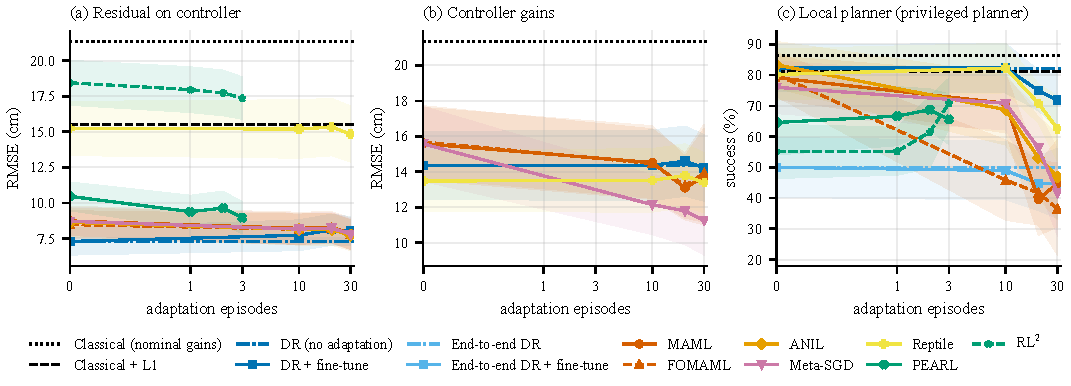
\includegraphics[width=\textwidth]{figures/adaptation_curves.pdf}
\caption{Adaptation pays off when it tunes classical gains (b), barely moves a learned residual (a), and at the meta-trained step size degrades learned navigation planners (c). Held-out tasks; mean and 95\% interval over tasks and seeds; horizontal lines are methods that do not adapt. A stage is one update from 10 episodes for the gradient-based methods and one more episode of experience for PEARL and RL$^2$. End-to-end planners are omitted from (c); see Table~\ref{tab:nav}.}
\label{fig:curves}
\end{figure*}

\subsection{Learning versus classical adaptation}\label{sec:rq1}

\textbf{A learned residual roughly halves the error of classical adaptation.} On held-out tasks the nominal geometric controller tracks with \valResClassicalPost\,cm RMSE and L1 augmentation with \valResLonePost\,cm (Table~\ref{tab:tracking}). A DR residual trained over all tasks reaches \valResDrPost\,cm without any adaptation. To make sure L1 is not a weak baseline, we grid-searched its predictor pole and filter bandwidth on training tasks (best: \valLoneTunedPole\,s$^{-1}$, \valLoneTunedCutoff\,rad/s); tuning lowers its held-out error only from \valLoneDefaultTest\ to \valLoneTunedTest\,cm on a common set of episodes, still about twice the residual's.

\subsection{Where meta-learning adds value}\label{sec:rq2}

\textbf{On top of a residual, meta-learning adds little.} MAML, FOMAML, ANIL and Meta-SGD start slightly worse than DR (\valResMamlPre, \valResFomamlPre, \valResAnilPre\ and \valResMetasgdPre\,cm) and improve with 30 adaptation episodes to \valResMamlPost, \valResFomamlPost, \valResAnilPost\ and \valResMetasgdPost\,cm, within the interval of DR's \valResDrPost\,cm (Fig.~\ref{fig:curves}a). With the same training budget as DR (Sec.~\ref{sec:learners}), they end where DR starts. Fine-tuning DR with PPO makes it slightly worse (\valResDrftPost\,cm), and Reptile trails at \valResReptilePost\,cm. Of the context-based methods, PEARL adapts from far less data (\valResPearlPre\ to \valResPearlPost\,cm with three episodes of context) but does not reach the gradient methods; RL$^2$ is the weakest learned residual (\valResRltwoPost\,cm).

\textbf{Adapting the classical gains is where meta-learning pays off.} When the policy chooses the controller's seven gains (Combination 2), every MAML-family method improves markedly with adaptation: Meta-SGD from \valGainMetasgdPre\ to \valGainMetasgdPost\,cm, MAML to \valGainMamlPost\,cm and FOMAML to \valGainFomamlPost\,cm, while gains tuned by DR stay at \valGainDrPost\,cm, or \valGainDrftPost\,cm with fine-tuning (Fig.~\ref{fig:curves}b). Paired over the same \valGainPairedN\ task--seed combinations, Meta-SGD improves on fine-tuned DR gains by \valGainPairedDiff\,cm (95\% bootstrap interval \valGainPairedLo--\valGainPairedHi\,cm) and wins on \valGainPairedWin\% of pairs. Adapted gains remain above the learned residual's error, but a seven-dimensional gain vector is a far smaller, more interpretable and more easily bounded object to adapt on a real vehicle.

\subsection{Adaptation inside the navigation stack}\label{sec:rq3}

\begin{table*}[t]
\centering
\caption{Navigation in unseen rooms. The classical local planner is the most reliable on the full stack, and gradient-based adaptation at the meta-trained step size lowers learned planners' success. Success and collision rates before and after adapting, with the privileged planner (3 stages) and on the full online-mapping stack (1 stage), and OOD success. \valSeedsNav\ training seeds; each episode in its own unseen room. Bold: best in column.}
\label{tab:nav}
\footnotesize
% generated by figures_scripts/navigation_table.py; do not edit
\begin{tabular}{@{}llrrrrrrr@{}}
\toprule
 & & \multicolumn{3}{c}{Privileged planner (96 rooms)} & \multicolumn{3}{c}{Full stack (48 rooms)} & OOD \\
\cmidrule(lr){3-5}\cmidrule(lr){6-8}
Method & Data & Before & After & Coll. & Before & After & Coll. & After \\
 & (ep.) & (\%) & (\%) & (\%) & (\%) & (\%) & (\%) & (\%) \\
\midrule
\multicolumn{9}{@{}l}{\emph{Classical}} \\
Classical (nominal gains) & 0 & \textbf{83} & \textbf{83} & \textbf{14} & \textbf{73} & \textbf{73} & \textbf{7} & 16 \\
Classical + L1 & 0 & 77 & 77 & 21 & \textbf{73} & \textbf{73} & 9 & 8 \\
\multicolumn{9}{@{}l}{\emph{Non-meta learned}} \\
DR (no adaptation) & 0 & 72 & 72 & 28 & 44 & 44 & 56 & 13 \\
DR + fine-tune & 30 & 72 & 71 & 29 & 44 & 50 & 50 & \textbf{17} \\
End-to-end DR & 0 & 52 & 52 & 48 & 51 & 51 & 49 & 10 \\
End-to-end DR + fine-tune & 30 & 52 & 46 & 54 & 51 & 47 & 53 & 16 \\
\multicolumn{9}{@{}l}{\emph{Gradient meta-learning (warm-started)}} \\
MAML & 30 & 73 & 36 & 60 & 46 & 32 & 67 & 8 \\
FOMAML & 30 & 76 & 31 & 69 & 53 & 31 & 69 & 5 \\
ANIL & 30 & 76 & 35 & 65 & 49 & 45 & 55 & 8 \\
Meta-SGD & 30 & 71 & 49 & 50 & 46 & 48 & 51 & 6 \\
Reptile & 30 & 72 & 71 & 29 & 46 & 47 & 53 & 14 \\
\multicolumn{9}{@{}l}{\emph{Context meta-learning (from scratch)}} \\
PEARL & 3 & 70 & 71 & 26 & 50 & 55 & 42 & 9 \\
RL$^2$ & 3 & 60 & 55 & 45 & 34 & 39 & 60 & 8 \\
\bottomrule
\end{tabular}

\end{table*}

\textbf{Gradient-based adaptation degrades learned planners at the meta-trained step size.} With the privileged planner, the warm-started MAML-family planners lose success as they adapt: MAML from \valNavMamlPre\% to \valNavMamlPost\%, FOMAML from \valNavFomamlPre\% to \valNavFomamlPost\%, ANIL from \valNavAnilPre\% to \valNavAnilPost\% and Meta-SGD from \valNavMetasgdPre\% to \valNavMetasgdPost\% (Table~\ref{tab:nav}, Fig.~\ref{fig:curves}c), with collisions rising as success falls. The decline already appears after the single update they were meta-trained for (MAML: \valNavMamlStageOne\%), so it is not only extrapolation. Methods that adapt conservatively stay flat: Reptile (\valNavReptilePre\% to \valNavReptilePost\%) and DR with fine-tuning (\valNavDrftPre\% to \valNavDrftPost\%) take small Adam steps, and PEARL (\valNavPearlPre\% to \valNavPearlPost\%) takes none. RL$^2$ does not improve with experience (\valNavRltwoPre\% to \valNavRltwoPost\%).

\begin{table}[t]
\centering
\caption{The navigation decline is a step-size effect. Success by adaptation stage and final collision rate with the inner step scaled from its meta-trained value, or with 30 instead of 10 episodes per update. Privileged planner, 16 held-out tasks in unseen rooms, seed-0 checkpoints.}
\label{tab:stepsize}
\footnotesize
% generated by figures_scripts/step_size_table.py; do not edit
\begin{tabular}{@{}lrrrrr@{}}
\toprule
 & \multicolumn{4}{c}{Success by stage (\%)} & Coll. \\
\cmidrule(lr){2-5}
Configuration & 0 & 1 & 2 & 3 & (\%) \\
\midrule
MAML, meta-trained step & 69 & 58 & 39 & 25 & 69 \\
MAML, step $\times$0.3 & 69 & 75 & 64 & 66 & 34 \\
MAML, step $\times$0.1 & 69 & 72 & 70 & 72 & 28 \\
MAML, 30 ep./stage & 69 & 75 & 62 & 64 & 36 \\
Meta-SGD, learned steps & 67 & 64 & 50 & 38 & 58 \\
Meta-SGD, steps $\times$0.3 & 67 & 69 & 67 & 73 & 27 \\
Meta-SGD, steps $\times$0.1 & 67 & 70 & 69 & 70 & 30 \\
\bottomrule
\end{tabular}

\end{table}

\textbf{The decline is a step-size and data-budget effect.} Scaling the inner step at test time (Table~\ref{tab:stepsize}) shows that the drop occurs at the meta-trained step with 10 episodes per update (MAML: \valStepMamlOnePre\% to \valStepMamlOnePost\%). With a 10$\times$ smaller step MAML holds at \valStepMamlTenthPost\% (Meta-SGD: \valStepMetasgdTenthPost\%), and with three times more episodes per update at the original step it holds at \valStepMamlDataPost\%. Smaller steps prevent the damage but buy little: success stays within a few points of its pre-adaptation level. Step sizes meta-learned for one task family therefore do not transfer to the sparse, high-variance returns of navigation, and on a real vehicle they should be scaled down or paired with more data per update.

\textbf{On the full stack, the classical planner is the most reliable.} With a map built in flight and A* replanning, the classical local planner reaches the goal in \valNavClassicalFullPost\% of \valNavFullFlights\ flights in unseen rooms with \valNavClassicalFullColl\% collisions, and L1 augmentation does not change this (\valNavClassicalloneFullPost\%). The learned planners reach \valNavFullLearnedLo--\valNavFullLearnedHi\% with \valNavFullCollLo--\valNavFullCollHi\% collisions. Learned planners also lose far more than the classical planner when the privileged planner is replaced by the online map (DR: \valNavDrPre\% to \valNavDrFullPost\%; classical: \valNavClassicalPre\% to \valNavClassicalFullPost\%). They were trained against carrots from a perfect map, and the online map's late-discovered obstacles and replanned paths fall outside that training distribution. Fig.~\ref{fig:flight} shows a recorded classical flight.

\textbf{The planner helps a learned policy only when the map is good.} With the privileged planner, the DR planner that follows the carrot beats the end-to-end DR planner that sees only the goal direction (\valNavDrPre\% vs \valNavEtoePre\%). On the full stack the order flips (\valNavDrFullPost\% vs \valNavEtoeFullPost\%): the end-to-end planner never depended on a map, so it loses nothing when the map is imperfect.

\begin{figure}[t]
\centering
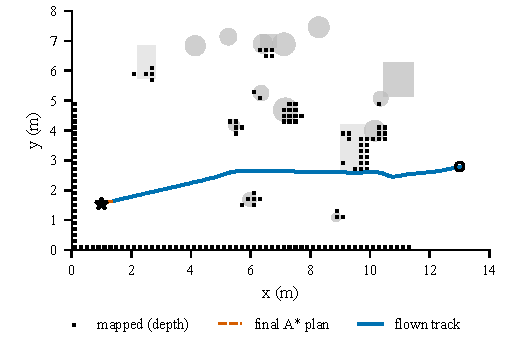
\includegraphics[width=\columnwidth]{figures/example_flights.pdf}
\caption{The classical stack maps an unseen room from its depth camera and reaches the goal. Grey: true obstacles (paler boxes hang overhead and are flown under); black: voxels mapped by the end of the flight; dashed: final A* plan; blue: flown track from start (circle) to goal (star).}
\label{fig:flight}
\end{figure}

\subsection{Beyond the training distribution}\label{sec:rq4}

\textbf{Every method fails out of distribution, and learned residuals crash more.} On the OOD tasks, which combine heavier payload, weaker motors, stronger wind and longer latency, no tracking method gets below \valOodRmseMin\,cm RMSE and no navigation method exceeds \valNavOodMax\% success. Learned residuals crash in \valResOodCrashLearnedLo--\valResOodCrashLearnedHi\% of OOD episodes, against \valResClassicalOodCrash\% for the nominal controller, and three adaptation stages change OOD error by at most \valOodAdaptMaxDelta\,cm. The pattern already appears just outside the training ranges: on a milder split that exceeds each range only slightly, the DR residual still tracks better than the nominal controller (\valMildDrRmse\ vs \valMildClassicalRmse\,cm), but DR and MAML-family residuals crash in \valMildResidCrashLo--\valMildResidCrashHi\% of episodes against \valMildClassicalCrash\%. Learned residuals thus trade safety margin for accuracy at the edge of the envelope, and the plain classical controller degrades most gracefully.

\section{Real-World Platform and Test Plan}\label{sec:platform}

The stack needs a flight controller that accepts CTBR or velocity setpoints from a companion computer at 50\,Hz or more, a depth camera, onboard compute for mapping and planning, and a vehicle that is safe in a netted cage. Table~\ref{tab:platforms} compares indoor research platforms in the \$1--3k range, from manufacturer pages checked on 2026-10-05.

\begin{table}[t]
\centering
\caption{Candidate platforms. Only the X500 build is in stock, within budget, and carries a depth camera that matches the simulator. Status from manufacturer stores on 2026-10-05.}
\label{tab:platforms}
\scriptsize
\setlength{\tabcolsep}{3pt}
\begin{tabular}{@{}lllll@{}}
\toprule
Platform & Mass & Depth & CTBR & Status \\
\midrule
X500 V2 build$^\dagger$ & $\approx$2.0\,kg & D435i & PX4 & in stock \\
Crazyflie 2.1 Brushless & 37\,g & none & partial & listed \\
Starling 2 & 285\,g & ToF & PX4 & unavailable new \\
Starling 2 Max & 566\,g & ToF (C29 only) & PX4 & over budget \\
PX4 Vision V1.5 & 893\,g$^*$ & discontinued & PX4 & sold out \\
\bottomrule
\multicolumn{5}{@{}l}{$^\dagger$Holybro X500 V2 + Jetson Orin Nano Super + D435i. $^*$Without battery.}
\end{tabular}
\end{table}

We recommend a Holybro X500 V2 with a Jetson Orin Nano Super and a RealSense D435i, about \$1.6--2.0k in parts. PX4's offboard mode takes body rates and collective thrust directly, the policies' own action space. The D435i is the camera the simulator models, and the X500 is PX4's reference airframe, so its simulator parameters come from a published model. The cost of this choice is a 2\,kg vehicle with 10-inch propellers, which must fly inside a netted cage. The Crazyflie is the safest vehicle for checking that low-level control transfers, but it cannot carry a depth camera.

The test plan has five stages, each gated by the previous one: (0) system identification of mass, inertia, thrust curve and motor lag to replace our estimates; (1) hover with the policy in the loop under motion capture; (2) trajectory tracking with known added payloads, compared with the simulator; (3) known foam obstacles with live depth mapping; (4) an unknown room with onboard visual-inertial odometry only. Safety layers include an RC kill switch, PX4 geofence, offboard-loss failsafe, and a watchdog that falls back to hold if commands arrive late.

\section{Limitations}\label{sec:limitations}

All results are in simulation; no real flights have been made. The thrust-to-weight ratio, motor lag and drag of the simulated vehicle are estimates. The aerodynamics are simple (linear drag, no ground effect or rotor drag), the depth model lacks texture- and lighting-dependent stereo artefacts, and state estimation is perfect. Compute was a single shared CPU, which limited seeds (\valSeedsRes\ for the residual, \valSeedsGain\ for gains, \valSeedsNav\ for navigation) and training length; the step-size study uses one seed. On navigation, the gradient-based learners start from the trained DR planner while PEARL and RL$^2$ train from scratch, and PEARL and RL$^2$ were trained on fewer environment steps (Sec.~\ref{sec:learners}), so their comparison with the others is confounded. Learned planners were trained with a privileged planner and tested on the online stack, which explains part of their full-stack gap. The MAML implementations ignore the dependence of the pre-adaptation sampling distribution on the parameters. Finally, our OOD tasks are harsh enough that every method fails on them.

\section{Conclusion}\label{sec:conclusion}

Combining meta-learning with a classical quadrotor stack at three insertion points, we found that a robust learned residual captures most of the tracking benefit without meta-learning, that meta-learning pays off most when it tunes classical gains, and that gradient-based adaptation can make learned navigation planners less safe, while a recurrent policy improved with experience. A classical local planner on an online map was the most reliable navigator in unseen rooms, and every method failed beyond the training distribution. These results argue for keeping classical components in the loop and adapting their parameters, and for testing adaptation methods on out-of-distribution conditions before trusting them on a real vehicle, which is the next step on the platform we recommend.

\section*{Acknowledgment}
The simulator, learning algorithms, experiments, benchmark, figures and table scripts, and the text of this paper were produced with an AI coding assistant (Claude Code, Anthropic) working under the author's direction. Citation metadata were checked against arXiv and Crossref by script. The author reviewed the results and is responsible for all claims.


\label{pw:mainend}
\bibliographystyle{IEEEtran}
\bibliography{refs}

\end{document}
